\chapter{Solidity Design Pattern Analyzer}
\begin{figure}[H]
	\centering
	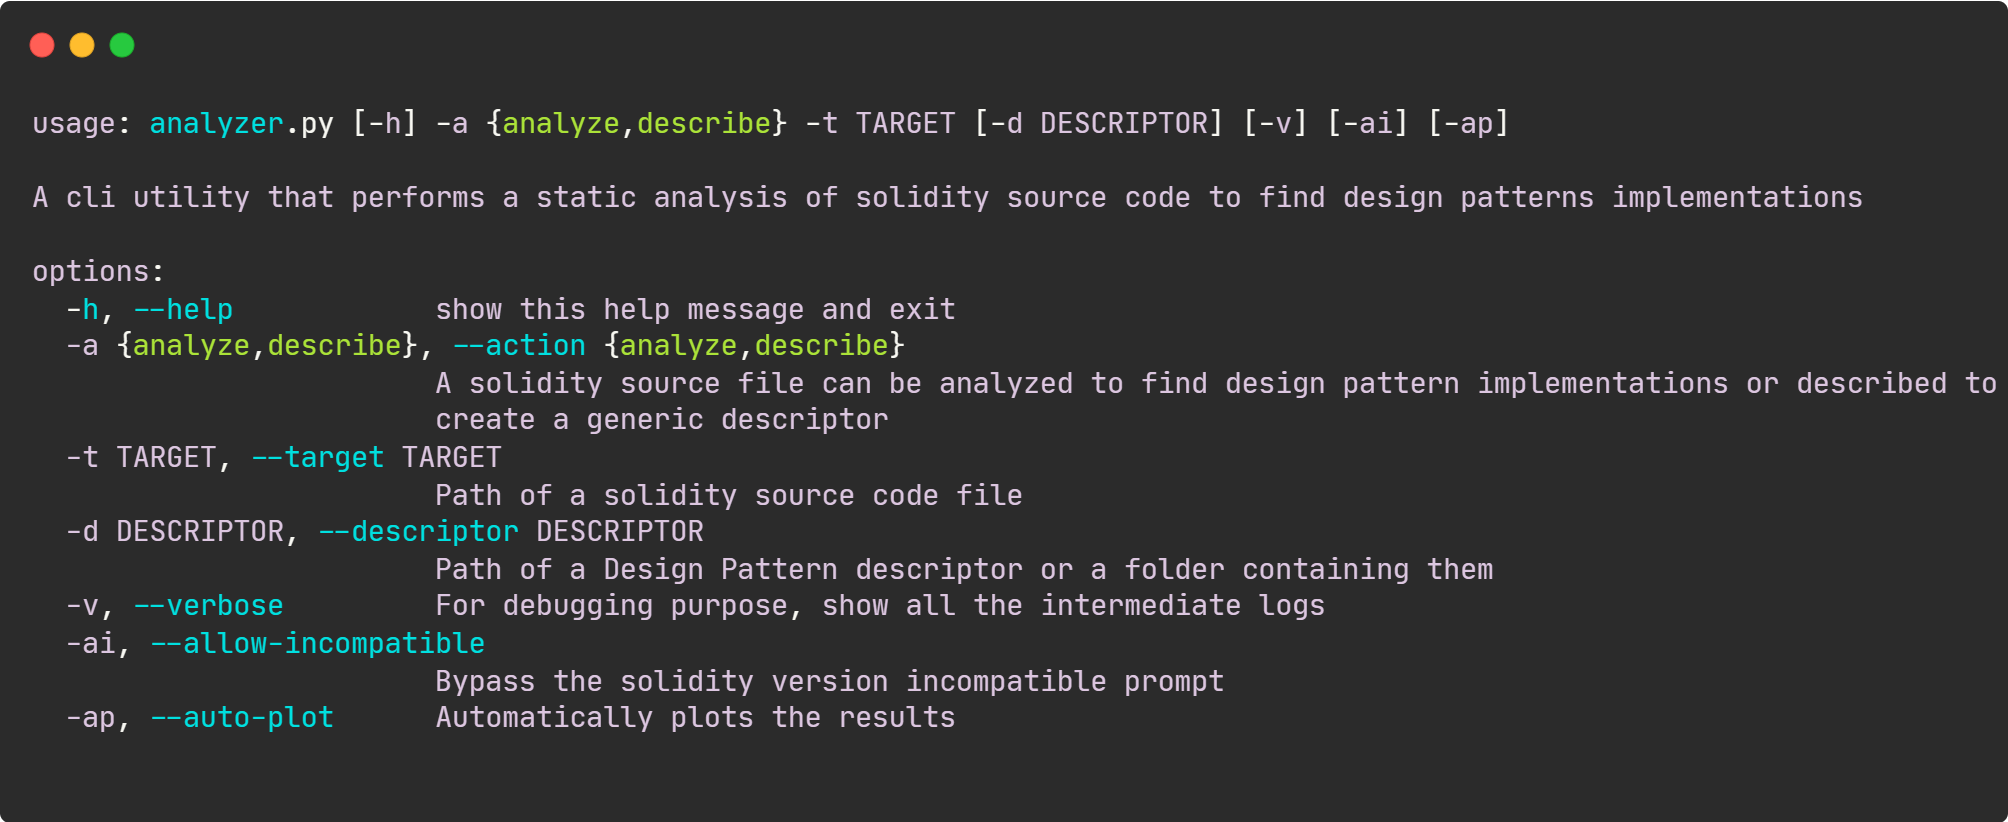
\includegraphics[width=\linewidth]{analyzer-tooltip}
	\caption{Manuale delle istruzioni di Analyzer}
	\label{analyzer-help-tip}
\end{figure}
L'applicativo software sviluppato è denominato \textit{"Solidity Design Pattern Analyzer"}, a cui, per semplicità, sarà fatto riferimento tramite l'abbreviazione \textit{"Analyzer"}.\\
\newline
Analyzer è un programma a riga di comando sviluppato in Python 3, e quindi supportato su MacOS, Linux e Windows, che prende in input il codice sorgente di un contratto, esegue una computazione e restituisce i risultati all'utente.\par
Lo scopo principale di Analyzer è automatizzare il processo di analisi statica del codice sorgente di uno smart-contract con l'obiettivo di individuare quali design pattern siano stati utilizzati.\par
Secondariamente, è possibile utilizzare Analyzer per \textit{descrivere} uno smart-contract, ovvero estrarre, tramite il processo di analisi statica, le informazioni utili a rappresentare un design pattern.

\section{Uso del programma}
Analyzer fa uso di librerie esterne, come ad esempio \textit{python-jsonschema}\cite{JSON-Schema} e \textit{matplotlib}. Per questo motivo, prima di poter utilizzare il programma è necessario installare tramite \textit{"pip"}, il package installer di Python, le dipendenze in uno dei seguenti modi:
\begin{itemize}
	\item \textit{Global Package}: installare le dipendenze direttamente nel sistema, diventando di fatto globali e accessibili da qualunque script Python eseguito nel sistema;
	\item \textit{Virtual Environment}: creare un ambiente virtuale in cui installare le dipendenze;
\end{itemize}
Una volta installate le dipendenze, per utilizzare Analyzer è necessario fornire una serie di parametri, qui elencati:
	\begin{table}[H]
	\centering
	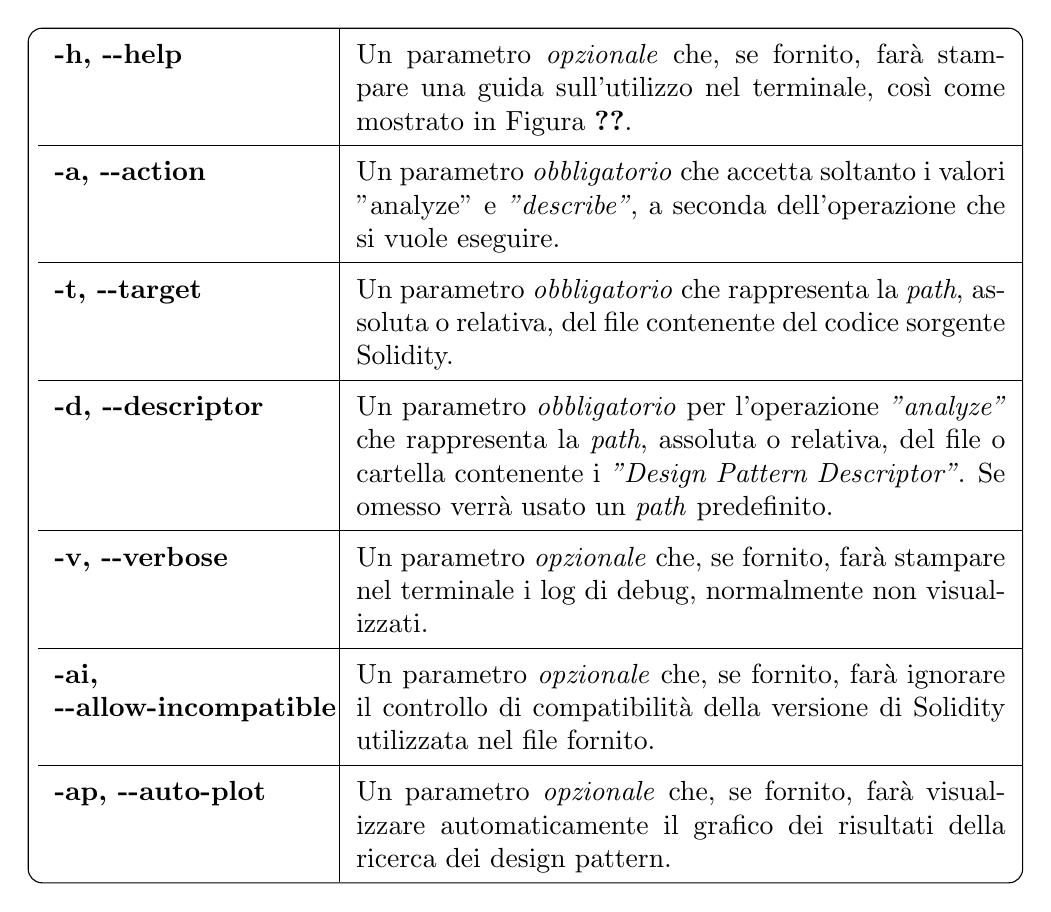
\begin{tikzpicture}
		\node (table) [inner sep=0pt] {
			\def\arraystretch{1.5}
			\begin{tabular}{p{0.28\linewidth} | p{0.68\linewidth}}
				\textbf{-h, -\/-help} & {Un parametro \textit{opzionale} che, se fornito, farà stampare una guida sull'utilizzo nel terminale, così come mostrato in \mbox{Figura} \ref{analyzer-help-tip}.} \\ \hline
				\textbf{-a, -\/-action} & {Un parametro \textit{obbligatorio} che accetta soltanto i valori \textit\mbox{"analyze"} e \textit{"describe"}, a seconda dell'operazione che si vuole eseguire.} \\ \hline
				\textbf{-t, -\/-target} & {Un parametro \textit{obbligatorio} che rappresenta la \textit{path}, assoluta o relativa, del file contenente del codice sorgente Solidity.} \\ \hline
				\textbf{-d, -\/-descriptor} & {Un parametro \textit{obbligatorio} per l'operazione \textit{"analyze"} che rappresenta la \textit{path}, assoluta o relativa, del file o cartella contenente i \textit{"Design Pattern Descriptor"}. Se omesso verrà usato un \textit{path} predefinito.} \\ \hline
				\textbf{-v, -\/-verbose} & {Un parametro \textit{opzionale} che, se fornito, farà stampare nel terminale i log di debug, normalmente non visualizzati.} \\ \hline
				\textbf{-ai, \mbox{-\/-allow-incompatible}} & {Un parametro \textit{opzionale} che, se fornito, farà ignorare il controllo di compatibilità della versione di Solidity utilizzata nel file fornito.} \\ \hline
				\textbf{-ap, -\/-auto-plot} & {Un parametro \textit{opzionale} che, se fornito, farà visualizzare automaticamente il grafico dei risultati della ricerca dei design pattern.} \\
			\end{tabular}
		};
		\draw [rounded corners=.5em] (table.north west) rectangle (table.south east);
	\end{tikzpicture}
	\caption{Descrizione dei parametri di Analyzer}
\end{table}
\noindent Il parametro \textit{"action"} determina che tipo di operazione Analyzer debba eseguire sul file fornito:
\begin{itemize}
	\item \textit{analyze}: effettua la ricerca dell'utilizzo di design pattern e restituisce i risultati in formato JSON, opzionalmente è possibile visualizzare un grafico riassuntivo;
	\item \textit{describe}: estrae le informazioni utili a rappresentare un design pattern e restituisce i risultati in formato JSON, costituendo un \textit{descriptor};
\end{itemize}
Entrambe le operazioni si basano sulla tecnica di analisi statica.\par
Per esempio, volendo analizzare uno smart-contract al fine di individuare l'utilizzo dell'\textit{Ownership} pattern è necessario eseguire il comando:
\begin{lstlisting}[language=bash]
	$ python analyzer.py -a analyze -t ./source_code.sol -d ./Ownership_descriptor.json
\end{lstlisting}

\section{Applicazione dell'analisi statica}
Per eseguire l'analisi statica del codice sorgente fornito, Analyzer fa uso di una libreria esterna denominata \textit{"python-solidity-parser"}, che implementa un \textit{parser}, sperimentale e abbastanza acerbo, per il linguaggio di programmazione Solidity.\par
Tramite l'utilizzo del parser si effettua un controllo di correttezza sintattica del codice sorgente e si costruisce l'\textit{albero sintattico astratto} (\textit{AST}), una rappresentazione strutturata e gerarchica della sintassi del programma. Gli elementi del codice sono rappresentati come nodi dell'albero, dove ogni nodo rappresenta una porzione del codice e i suoi figli rappresentano porzioni più piccole e specifiche.
\newline

\noindent Con l'obiettivo di ottenere un sistema flessibile e facilmente estendibile, senza dover effettuare modifiche al codice sorgente di Analyzer, si è deciso di implementare, quando possibile, controlli generici.\par
L'utilizzo di controlli generici, con parametri configurabili, permette di definire un'unica logica applicabile alla ricerca di design pattern differenti.\par
Tale soluzione non è, però, sempre applicabile, infatti per specifici design pattern si è preferito implementare controlli specializzati al loro rilevamento.

\subsection{Controlli generici}
I controlli generici implementano la ricerca e disamina di elementi comuni, come ad esempio un confronto o l'utilizzo di modifier.\par
Viene esplorato l'albero sintattico astratto al fine di individuare i nodi di interesse, successivamente vengono estratte le informazioni utili e confrontate, mediante confronti \textit{case-insensitive} fra stringhe, con i parametri forniti.\par
Analyzer comprende i seguenti controlli generici: \textit{"comparison"}, \textit{"enum\textunderscore definition"}, \textit{"event\textunderscore emit"}, \textit{"fn\textunderscore call"}, \textit{"fn\textunderscore definition"}, \textit{"fn\textunderscore return\textunderscore parameters"}, \textit{"inheritance"}, \textit{"modifier"} e \textit{"state\textunderscore toggle"}.
\subsubsection{Comparison}
Questo controllo individua l'esecuzione di un'\textit{operazione di confronto} fra due operandi. Un'operazione di confronto fa uso di uno dei seguenti operatori: (==, !=, \textgreater, \textgreater =, \textless, \textless =).\par
Definita un'operazione di confronto, verrà automaticamente presa in considerazione anche quella con l'inversione dell'operatore equivalente.\par
Data la libertà implementativa, è possibile definire più di un'operazione di confronto, il controllo restituirà esito positivo al primo \textit{match} eseguito con successo.
Segue un esempio di parametrizzazione del controllo \textit{comparison}:
{\begin{lstlisting}[language=json, caption={Parametrizzazione del controllo Comparison}]
{
	"check_type": "comparison",
	"binary_operations": [
	{
		"operator": ">",
		"operand_1": "bilancio",
		"operand_2": "prelievo"
	}]
}\end{lstlisting}}
\noindent Tale controllo darà esito positivo per i confronti: \textit{bilancio\textgreater prelievo} e \textit{prelievo\textless bilancio}.\par
La verifica degli operandi viene effettuata assumendo che i parametri forniti debbano essere sotto-stringhe dei rispettivi operandi.

\subsubsection{Enum Definition}
Questo controllo individua la definizione di variabili di stato di tipo \textit{enum} denominati in modo specifico.\par
Possono essere forniti più nomi, il controllo restituirà esito positivo al primo \textit{match} eseguito con successo.
Segue un esempio di parametrizzazione:
{\begin{lstlisting}[language=json, caption={Parametrizzazione del controllo Enum Definition}]
{
	"check_type": "enum_definition",
	"enum_names": ["colori"]
}\end{lstlisting}}
\noindent Tale controllo darà esito positivo se all'interno del contratto è stato definito un \textit{enum} denominato \textit{"colori"}.\par
La verifica del nome dell'\textit{enum} viene effettuata assumendo che quest'ultimo sia contenuto nella lista dei parametri forniti. Si può definire un parametro come \textit{wildcard}, o sotto-stringa, concatenando il parametro stesso al simbolo '*': \textit{"colori*"}.


\subsubsection{Event emit}
Questo controllo individua l'emissione di di un evento.\par
Possono essere forniti molteplici nomi di eventi, il controllo restituirà esito positivo al primo \textit{match} eseguito con successo.
Segue un esempio di parametrizzazione:
{\begin{lstlisting}[language=json, caption={Parametrizzazione del controllo Event Emit}]
{
	"check_type": "event_emit",
	"enum_names": ["request*"]
}\end{lstlisting}}
\noindent Tale controllo darà esito positivo se all'interno del contratto viene emesso un evento il cui nome contiene la sotto-stringa \textit{"request"}.\par
Analogamente al controllo \textit{enum definition}, è possibile fornire come nome anche una stringa specifica.

\subsubsection{Function Call}
Questo controllo individua la chiamata di una funzione, con la possibilità di specificare o meno i suoi parametri.\par
Possono essere fornite svariate chiamate di funzione, il controllo restituirà esito positivo al primo \textit{match} eseguito con successo.
Segue un esempio di parametrizzazione:
{\begin{lstlisting}[language=json, caption={Parametrizzazione del controllo Function Call}]
{
	"check_type": "fn_call",
	"callable_function": ["require(*any*)"]
}\end{lstlisting}}
\noindent Tale controllo darà esito positivo se all'interno del contratto viene eseguita la funzione \textit{require} con qualunque tipo di parametro.\par
La stringa \textit{"*any*"} rappresenta una \textit{wildcard}, è possibile sostituirla con i parametri \textit{esatti} della funzione.

\subsubsection{Function Definition}
Questo controllo individua la definizione di una funzione denominata in modo specifico.\par
Possono essere forniti più nomi di funzione, il controllo restituirà esito positivo al primo \textit{match} eseguito con successo.
Segue un esempio di parametrizzazione:
{\begin{lstlisting}[language=json, caption={Parametrizzazione del controllo Function Definition}]
{
	"check_type": "fn_definition",
	"fn_names": ["commit", "reveal", "tracecommit"]
}\end{lstlisting}}
\noindent Tale controllo darà esito positivo se all'interno del contratto è stato definita una funzione il cui nome è presente nella lista nomi forniti.\par
Analogamente agli altri controlli, si può fornire come parametro una \textit{wildcard}, o sotto-stringa.

\subsubsection{Function Return Parameters}
Questo controllo individua la definizione di una funzione che ritorna una specifica serie di variabili.\par Possono essere forniti molteplici variabili di ritorno, specificando per ognuna il tipo e la collocazione nello storage, il controllo restituirà esito positivo solo se esiste una funziona che ritorni almeno tutte le variabili fornite come parametro.
Segue un esempio di parametrizzazione:
{\begin{lstlisting}[language=json, caption={Parametrizzazione del controllo Function Return Parameters}]
{
	"check_type": "fn_return_parameters",
	"parameters_list": [
	{
		"storage_location": "memory",
		"type": "ElementaryTypeName"
	}]
}\end{lstlisting}}
\noindent Tale controllo darà esito positivo se esiste una funzione che ritorna almeno un \textit{dato elementare} collocato in \textit{memory}.\par
Si può accettare qualunque collocazione dello storage ponendo come \textit{storage\textunderscore location} la \textit{wildcard} "*".

\subsubsection{Inheritance}
L'ereditarietà è un concetto importante della \textit{programmazione orientata agli oggetti} (\textit{OOP}). Consente di creare nuove classi a partire da classi esistenti, ereditandone le proprietà e i comportamenti. Questo rende più semplice la creazione di nuove classi e la manutenzione del codice, poiché è possibile riutilizzare e modificare il codice esistente invece di creare tutto da zero.\par
Solidity supporta l'ereditarietà tra smart-contract, dove più contratti possono essere ereditati in un singolo contratto. Il contratto da cui gli altri contratti ereditano le caratteristiche è noto come \textit{contratto base}, mentre il contratto che eredita le caratteristiche è detto \textit{contratto derivato}:
\begin{itemize}
	\item Un \textit{contratto derivato} può accedere a tutti i membri non privati, comprese le variabili di stato, i funzioni interni e modifier;
	\item L'\textit{overriding} delle funzioni è consentitp a condizione che la firma della funzione rimanga la stessa;
	\item Si può chiamare la funzione di un contratto base usando la parola chiave \textit{super} o il nome del \textit{contratto base}.
\end{itemize}
Questo controllo individua la singola o multipla ereditarietà del contratto fornito e confronta il nome dei \textit{contratti base} ottenuti con una lista di nomi fornita come parametro.\par
Costituisce uno dei controlli più utilizzati in combinazione con gli altri, in quanto, supponendo l'utilizzo di libreria come \textit{OpenZeppelin}\cite{openzeppelin}, è più probabile ereditare le caratteristiche di un design pattern anziché implementarle da zero.\par
Possono essere forniti più nomi di \textit{contratti base}, il controllo restituirà esito positivo al primo \textit{match} eseguito con successo.
Segue un esempio di parametrizzazione:
{\begin{lstlisting}[language=json, caption={Parametrizzazione del controllo Inheritance}]
{
	"check_type": "inheritance",
	"parent_names": ["deprecatable"]
}\end{lstlisting}}
\noindent Tale controllo darà esito positivo se il contratto che si sta analizzando eredità le proprietà e le caratteristiche di un contratto denominato \textit{"Deprecatable"}.\par
Analogamente agli altri controlli, è possibile fornire come nome anche una \textit{wildcard}.

\subsubsection{Modifier}
Questo controllo individua la definizione o l'utilizzo di modifier denominati in modo specifico.\par
Possono essere forniti più nomi di \textit{modifier}, il controllo restituirà esito positivo al primo \textit{match} eseguito con successo.
Segue un esempio di parametrizzazione:
{\begin{lstlisting}[language=json, caption={Parametrizzazione del controllo Modifier}]
{
	"check_type": "modifier",
	"modifiers": ["when*", "after*"]
}\end{lstlisting}}
\noindent Tale controllo darà esito positivo se esiste almeno una funzione che utilizza almeno uno dei modifier forniti come parametro.\par
Analogamente agli altri controlli, è possibile fornire anche un nome specifico.

\subsubsection{State Toggle}
Questo controllo individua l'utilizzo di un interruttore software. L'interruttore è rappresentato da una variabile di stato \textit{booleana} e da una funzione che ne esegue il \textit{flip}.\par
Data la libertà implementativa, viene riconosciuto il \textit{flip} più comunemente utilizzato, basato sull'operatore di negazione (\textit{state\textunderscore bool = !state\textunderscore bool}).\par
Possono essere forniti più nomi di variabile, il controllo restituirà esito positivo al primo \textit{match} eseguito con successo.
Segue un esempio di parametrizzazione:
{\begin{lstlisting}[language=json, caption={Parametrizzazione del controllo Comparison}]
{
	"check_type": "state_toggle",
	"state_names": ["paused*"]
}\end{lstlisting}}
\noindent Tale controllo darà esito positivo se esistono una variabile di stato booleana che nel nome contiene \textit{"paused"} e un'istruzione di \textit{flip} relativa.\par
Analogamente agli altri controlli, è possibile fornire anche un nome specifico.

\subsection{Controlli specializzati}
I controlli specializzati implementano la ricerca e disamina di elementi specifici, difficilmente rappresentabili come elementi semplici, come ad esempio la distanza fra una funzione esterna e un assegnamento o il packing delle variabili.\par
Analyzer comprende i seguenti controlli specializzati: \textit{"check\textunderscore effects\textunderscore interaction"}, \textit{"eternal\textunderscore storage"}, \textit{"memory\textunderscore array\textunderscore building"}, \textit{"rejector"}, \textit{"relay"} e \textit{"tight\textunderscore variable\textunderscore packing"}
\subsubsection{Check Effects Interaction}
Questo controllo individua l'omonimo design pattern.\par Ricerca una chiamata alle funzioni esterne offerte da Solidity, ovvero l'utilizzo delle funzioni \textit{call()}, \textit{send()} e \textit{transfer()}, preceduta da un'istruzione di assegnamento.\par Al fine di affinare la probabilità di rilevamento e diminuire i casi falsi positivi, si è definita una distanza massima di cinque righe.
{\begin{lstlisting}[language=json, caption={Controllo Check Effects Interaction}]
{ "check_type": "check_effects_interaction" }\end{lstlisting}}

\subsubsection{Eternal Storage}
Questo controllo individua il \textit{Data Segregation} pattern, conosciuto anche come \textit{Eternal Storage}.\par Data la libertà implementativa, il controllo è incentrato sulla ricerca di \textit{mapping} e la definizione delle funzioni di supporto \textit{getter} e \textit{setter}.\par
Il nome delle funzioni di supporto è definito come il nome del mapping preceduto rispettivamente da \textit{"get"} e \textit{"set"}.\par
Nell'EVM, un mapping definito con visibilità \textit{pubblica} genera automaticamente un \textit{getter}, viene, perciò, gestito anche il caso in cui non vi sia l'esplicita definizione del \textit{getter}. 
{\begin{lstlisting}[language=json, caption={Controllo Eternal Storage}]
{ "check_type": "eternal_storage" }\end{lstlisting}}
	
\subsubsection{Memory Array Building}
Questo controllo individua l'omonimo design pattern.\par Ricerca la definizione di una funzione con modifier \textit{view} che ritorni un array collocato in \textit{memory}.
{\begin{lstlisting}[language=json, caption={Controllo Memory Array Building}]
{ "check_type": "memory_array_building" }\end{lstlisting}}
	
\subsubsection{Rejector}
Questo controllo individua l'omonimo design pattern.\par Verifica che il contratto fornito implementi \textit{solo} la funzione di \textit{fallback()} in cui viene eseguita la funzione \textit{revert()}.
{\begin{lstlisting}[language=json, caption={Controllo Rejector}]
{ "check_type": "rejector" }\end{lstlisting}}
	
\subsubsection{Relay}
Questo controllo individua sia il \textit{Relay} pattern sia il \textit{Register} pattern.\par Verifica che il contratto fornito implementi la funzione di \textit{fallback()} in cui viene eseguita la funzione \textit{delegatecall()}.
{\begin{lstlisting}[language=json, caption={Controllo Relay}]
{ "check_type": "relay" }\end{lstlisting}}
	
\subsubsection{Tight Variable Packing}
Questo controllo individua l'omonimo design pattern.\par Ricerca la definizione di una \textit{struct} contenente tipi di dati la cui somma delle dimensioni sia minore o uguale, quando possibile, a 32 byte.\par
Le \textit{struct} contenenti almeno un elemento di dimensione dinamica, come ad esempio array o numeri a virgola mobile, vengono scartate, in quanto non è possibile valutarne la dimensione a priori.
{\begin{lstlisting}[language=json, caption={Controllo Tight Variable Packing}]
{ "check_type": "tight_variable_packing" }\end{lstlisting}}

\section{Design Pattern Descriptor}
Stabiliti i controlli supportati da Analyzer, è possibile definire un \textit{Design Pattern Descriptor} come un \textit{oggetto JSON} contenente una raccolta di uno o più controlli opportunatamente parametrizzati al fine di individuare uno specifico design pattern.\par
Come esempio, si riporta il descriptor dell'\textit{Auto Deprecation} pattern:
	{\begin{lstlisting}[language=json, caption={Auto Deprecation Descriptor}, label={descriptor:auto_deprecation}]
{
	"name": "Auto Deprecation",
	"checks": [
	{
		"check_type": "inheritance",
		"parent_names": ["deprecatable"]
	},
	{
		"check_type": "modifier",
		"modifiers": ["willDeprecate", "whenDeprecated"]
	},
	{
		"check_type": "comparison",
		"binary_operations": [
		{
			"operator": ">",
			"operand_1": "timestamp",
			"operand_2": "expire"
		}]
	}]
}\end{lstlisting}}
\subsection{Affinamento dei parametri}
Per individuare un design pattern, la correttezza dei parametri dei controlli utilizzati è fondamentale. Un parametro troppo generico può causare dei falsi positivi, viceversa può ridurre le probabilità di riconoscimento.\par
Al fine di migliorare i parametri, estratti dai codici di riferimento riportati in \hyperref[appendix:codici]{Appendice}, si è analizzata la libreria \textit{OpenZeppelin Contracts}\cite{openzeppelin}, una libreria per lo sviluppo di smart-contract sicuri, costituita da una solida codebase verificata dalla comunità.\par Data la sua diffusione, si è utilizzato Analyzer per estrarre informazioni utili da utilizzare come ulteriori parametri.

\subsection{Validazione tramite JSONSchema}
Un descriptor descrive le caratteristiche principali di un design pattern e permette ad Analyzer di rilevarne l'utilizzo.\par 
Inoltre, allo scopo di rilevare nuovi design pattern, non riconosciuti da Analyzer, l'utente può definire, basandosi sui controlli supportati, nuovi descriptor.\\
\newline
Data la natura configurabile dei descriptor, nasce il rischio di incorrere in descriptor malformati o contenenti dati incoerenti, di conseguenza vi è la necessità di validarli in maniera semplice ed efficace.\par Per la convalida, Analyzer utilizza la libreria esterna denominata \textit{"python-jsonschema"} \cite{python-jsonschema} e lo schema \ref{appendix:json_schema}, riportato in \hyperref[appendix:codici]{Appendice}:
\begin{lstlisting}[language=Python, caption={Istruzione di validazione}]
jsonschema.validate(instance=descriptor_object, schema=self._descriptor_schema)
\end{lstlisting}
\noindent A scopo informativo, si riporta e commenta la porzione di schema che modella i dati del controllo \textit{"comparison"}, di cui vi è un utilizzo nel codice \ref{descriptor:auto_deprecation}:
{\begin{lstlisting}[language=json, caption={JSONSchema del controllo "comparison"}]
{
	"type": "object",
	"properties": { 
		"check_type": { "type": "string", "const": "comparison" },
		"binary_operations": {
			"type": "array",
			"items": [
			{
				"type": "object",
				"properties": { 
					"operator": { "type": "string" },
					"operand_1": { "type": "string" },
					"operand_2": { "type": "string" }
				},
				"required": [ "operator", "operand_1", "operand_2" ]
			}],
			"uniqueItems": true, "minItems": 1
		}
	},
	"required": [ "check_type", "binary_operations" ]},\end{lstlisting}}  
\noindent Questo modello descrive un oggetto JSON che deve soddisfare le seguenti regole:
\begin{itemize}
		\item {L'oggetto deve contenere le proprietà \textit{"check\textunderscore type"} e \textit{"binary\textunderscore operations"}, rispettivamente una \textit{stringa} di valore \textit{"comparison"} e un \textit{array JSON} di oggetti JSON, rappresentanti le operazioni binarie. Entrambe le proprietà sono obbligatorie;} 
		\item Un'operazione binaria è rappresentata da un oggetto JSON contenente le proprietà di tipo stringa \textit{"operator"}, \textit{"operand\textunderscore 1"} e \textit{operand\textunderscore 2}, tutte e tre obbligatorie;
		\item L'array JSON di operazioni binarie deve contenere almeno un elemento e tutti gli elementi devono essere distinti;
\end{itemize}
\section{Ricerca di Design Pattern}
Fornendo il valore \textit{"analyze"} come parametro \textit{"action"} viene effettuata la ricerca di design pattern nel codice sorgente fornito in input. L'esecuzione di questa operazione può essere essenzialmente suddivisa in tre fasi:
\begin{itemize}
	\item \textit{Bootstrap}: in questa fase vengono convalidati i parametri forniti dall'utente;
	\item \textit{Parsing e Analisi}: in questa fase vengono eseguiti il parsing del codice sorgente e la ricerca dei design pattern;
	\item \textit{Report dei risultati}: in questa fase vengono mostrati all'utente i risultati della ricerca, opzionalmente può essere mostrato un grafico riassuntivo;
\end{itemize}

\subsection{Fase di Bootstrap}
Nella fase di \textit{bootstrap} vengono verificati i parametri forniti dall'utente.\par
Viene verificata l'estensione dei file, affinché il parametro \textit{target} sia un file sorgente Solidity, e il parametro \textit{descriptor} sia un file \textit{json} o una cartella, contenente file \textit{json}.\par
Successivamente, i descriptor forniti vengono validati mediante lo schema \ref{appendix:json_schema}, riportato in \hyperref[appendix:codici]{Appendice}. I descriptor non validati vengono ignorati e non utilizzati nella fase successiva.\par
In caso di parametri invalidi, od omessi, viene restituito un messaggio d'errore esplicativo e, in caso di errore critico, viene terminato il processo.
\newpage
\subsection{Fase di Parsing e Analisi}
Nella fase di \textit{parsing e analisi}, mediante l'utilizzo del parser, viene effettuato un controllo di correttezza della sintassi e costruito l'albero sintattico astratto.\par
Successivamente, vengono eseguiti i controlli contenuti in ogni descriptor precedentemente convalidato, tenendo traccia di quali controlli hanno avuto esito positivo.\par
In caso di errori di sintassi all'interno del codice sorgente il processo viene terminato.

\subsection{Fase di Report dei risultati}
Nella fase di \textit{report dei risultati}, viene stampato sul terminale una sintesi dell'esito dei controlli eseguiti. Inoltre, tale sintesi viene salvata sul disco in formato JSON, nello stesso \textit{path} del file sorgente fornito in input.\par
L'esito positivo di uno dei controllo di un descriptor suggerisce, in quanto non è possibile fornire la certezza, che il design pattern rappresentato potrebbe essere in uso.\par
Opzionalmente, è possibile visualizzare la sintesi sotto forma di grafico.
\newline
Segue un esempio di sintesi in formato JSON:
{\begin{lstlisting}[language=json, caption={Report del codice di riferimento dell'Ownership}, label={report:ownership-text}]
{"Ownable":{
	"AccessRestriction":{"inheritance":false,"modifier":true},
	"AutoDeprecation":{"inheritance":false,"modifier":false,"comparison":false},
	"BalanceLimit":{"comparison":false},
	"CheckEffectsInteraction":{"check_effects_interaction":false},
	"CircuitBreaker":{
		"inheritance":false,
		"state_toggle":false,
		"fn_definition":false,
		"modifier":false
	},
	"CommitReveal":{
		"fn_call":false,
		"fn_definition":false,
		"event_emit":false
	},
	"EternalStorage":{"eternal_storage":false},
	"GuardCheck":{"fn_call":true},
	"MemoryArrayBuilding":{"memory_array_building":false},
	"Mortal":{"inheritance":false,"fn_call":false},
	"Mutex":{"inheritance":false,"modifier":false,"fn_definition":false},
	"Oracle":{"fn_call":false,"fn_definition":false,"event_emit":false},
	"Ownership":{"inheritance":false,"modifier":true,"comparison":true},
	"PullOverPush":{"inheritance":false,"fn_call":false},
	"Randomness":{"fn_call":false},
	"RateLimit":{"modifier":false,"inheritance":false},
	"Rejector":{"rejector":false},
	"Relay":{"inheritance":false,"relay":false},
	"SecureTransfer":{"fn_call":false},
	"StateMachine":{"modifier":false,"enum_definition":false,"fn_definition":false},
	"StringEquality":{"comparison":false},
	"TightVariablePacking":{"tight_variable_packing":false}
}}\end{lstlisting}
Il report testuale mostrato nel Codice \ref{report:ownership-text} può essere visualizzato in forma di grafico a barre:
\begin{figure}[H]
	\centering
	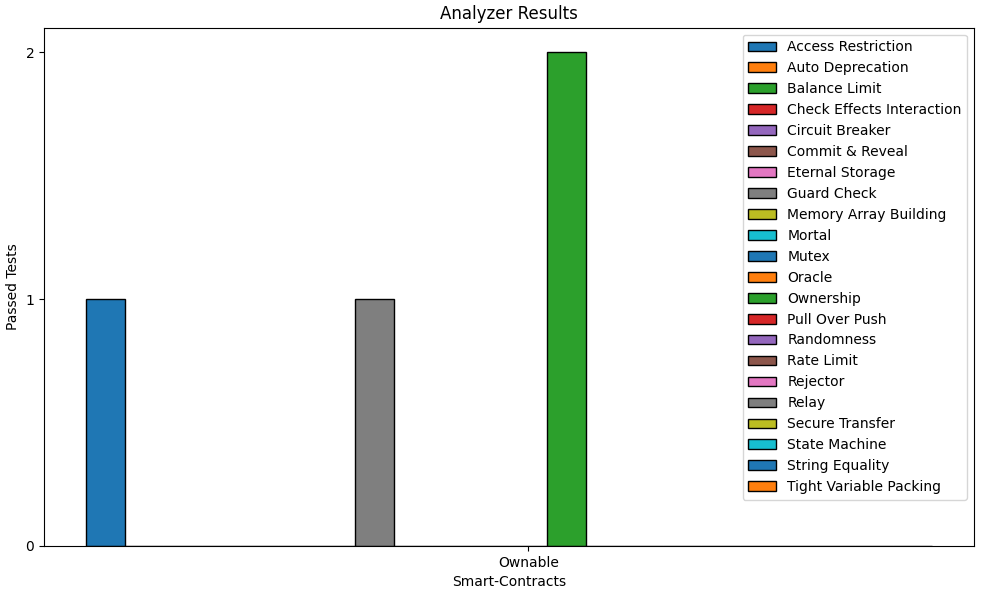
\includegraphics[width=\linewidth]{ownership-plot}
	\caption{Grafico a barre dell'analisi del codice di riferimento dell'Ownership}
\end{figure}

\section{Descrizione di uno smart-contract}
Fornendo il valore \textit{"describe"} come parametro \textit{"action"} viene effettuata descrizione dello smart-contract. \par
La descrizione consiste nel generare un descriptor con le informazioni utili estratte mediante l'analisi statica. Analogamente alla ricerca dei design pattern, l'esecuzione di questa operazione può essere similmente suddivisa in tre fasi:
\begin{itemize}
	\item \textit{Bootstrap}: in questa fase vengono convalidati i parametri forniti dall'utente;
	\item \textit{Parsing e Analisi}: in questa fase vengono eseguiti il parsing del codice sorgente e l'estrazione delle informazioni utili;
	\item \textit{Generazione del descriptor}: in questa fase generato e salvato il descriptor costituito dalle informazioni estratte;
\end{itemize}

\subsection{Fase di Bootstrap}
Analoga alla fase di \textit{bootstrap} della ricerca di design pattern.\par
Dato che l'operazione \textit{"describe"} non richiede alcun descriptor come input, viene verificata soltanto l'estensione del file sorgente Solidity.

\subsection{Fase di Parsing e Analisi}
Analogamente alla fase di \textit{parsing e analisi} della ricerca di design pattern, viene effettuato un controllo di correttezza della sintassi e costruito l'albero sintattico astratto.\par
Successivamente, viene eseguita una serie di funzioni di supporto per estrarre tutti i possibili parametri dei \textit{controlli generici}.\par
In caso di errori di sintassi all'interno del codice sorgente il processo viene terminato.

\subsection{Fase di Generazione del descriptor}
Nella fase di \textit{generazione del descriptor}, le informazioni utili estratte vengono raccolte in un descriptor, il quale viene salvato sul disco nello stesso \textit{path} del file sorgente fornito in input.\par
Segue il descriptor generato usando il codice \ref{appendix:ownership}:
{\begin{lstlisting}[language=json, caption={Report del codice di riferimento dell'Ownership}]
{
	"name": "Ownable",
	"checks": [
	{
		"check_type": "comparison",
		"binary_operations": [
		{
			"operator": "==",
			"operand_1": "_owner",
			"operand_2": "msg.sender"
		}
		]
	},
	{ "check_type": "modifier", "modifiers": [ "onlyowner" ] },
	{
		"check_type": "fn_call",
		"callable_function": [
			"address(0)",
			"require(_owner == msg.sender, \"ownable: caller is not the owner\")",
			"ownershiptransferred(address(0), _owner)"
		]
	},
	{ "check_type": "fn_definition", "fn_names": [ "constructor" ] },
	{ "check_type": "event_emit", "event_names": [ "ownershiptransferred" ] }]
}\end{lstlisting}